\newpage
\subsection{Fatigue verification of a notched plate}
	
	\paragraph{Problem} The plate in figure \ref{ex:fatigueplate} is subjected to a fluctuating axial loading from a minimum value $F_{min} = 1\,200N$ and a maximum of $F_{max} = 12\,000N$. The plate is made up of machined steel with a yield strength of $\sys = 380 MPa$ and tensile strength $\suts= 550MPa$; the mean (50\% failure probability) SN curve obtained under rotating bending is
	\[ \sigma_a = \begin{cases}
		330MPa &  N_f > 2\cdot 10^6 \\
		1\,220 N_f^{-0.09} \qquad & 10^4 < N_f < 2\cdot 10^6
	\end{cases} \]
	It is requested to determine the safety factors of the critical sections AA and BB for infinite fatigue life; the plate dimensions are $r=4mm, h = 32mm, b=5mm, d=12mm, H=48mm$. To determine the size factor $C_d$ use the equivalent diameter defined as
	\[ d_{eq} = \sqrt{\frac 4 \pi s w} \qquad \textrm{$s$: thickness, $w$: width} \]
	
	Then estimate the fatigue life when the plate is subjected to blocks of cycles of different amplitude listed in the table below:
	\begin{center}
		\rule{0.6\linewidth}{1.5pt} \\
		\begin{tabular}{ c M{2cm} M{2cm} M{2cm} }
			 &  $F_{min} [N]$ &  $F_{max}[N]$ & $n [\textrm{cycle}/h]$ \\ \hline
			\#1 & -1000 & 18000 & 2000 \\
			\#2 & -2000 & 26000& 1000 \\
			\#3 & 1200 & 28000 & 500 \\
			\#4 & 1000 & 30000 & 300 \\
			\#5 & 500 & 32500 & 100
		\end{tabular}
		\rule{0.6\linewidth}{1.5pt}
	\end{center}
	
	\begin{figure}[bh]
		\centering 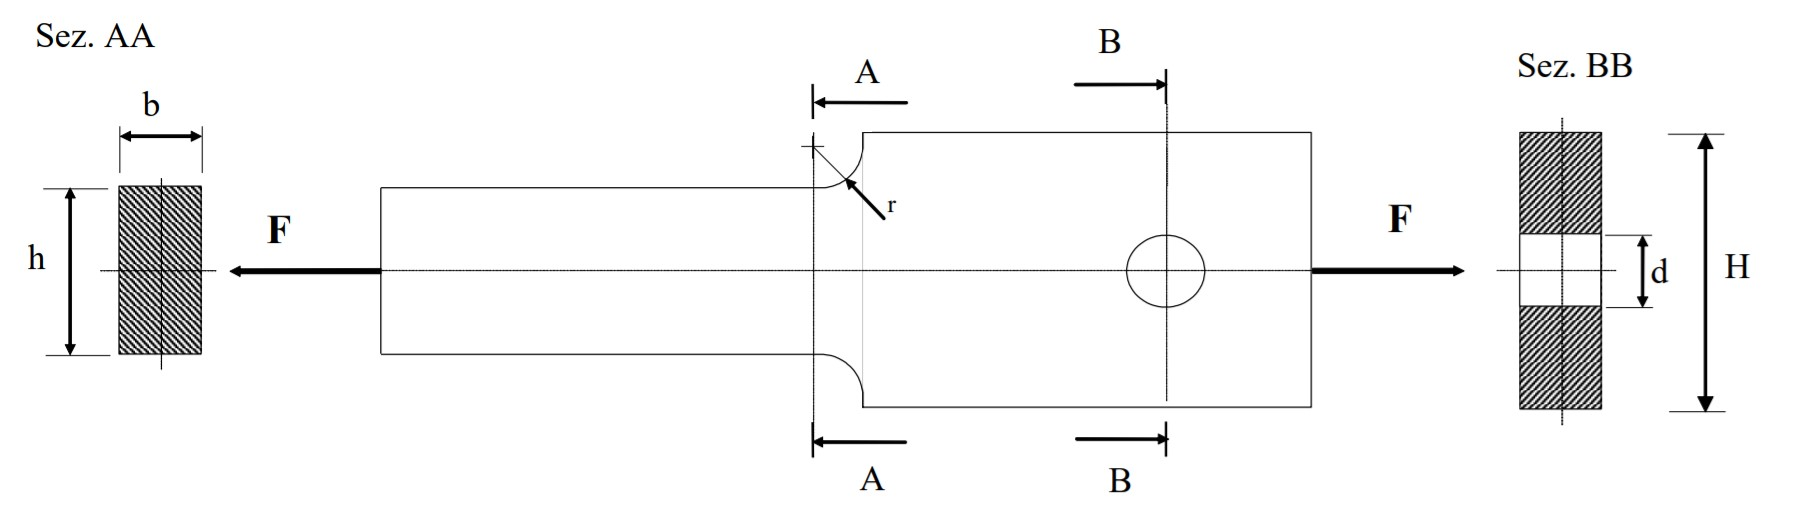
\includegraphics[width=13cm]{plate-fatigue}
		\caption{sketch of a notched plate subjected to fluctuating axial loading.} \label{ex:fatigueplate}
	\end{figure}
	
	\paragraph{Solution} The first thing to is reconvert the maximum/minimum values of the oscillating applied force into a mean value $F_m = \frac{F_{max}+F_{min}}{2} = 6\,600N$ and an oscillation $F_a = \frac{F_{max} - F_{min}}{2} = 5\,400N$. Dividing such values for the nominal area of the critical section gives so the mean/alternating stress components:
	\[ \sigma_{m,nom,AA} = \frac{F_m}{bh} = 41.25 MPa \qquad \sigma_{a,nom,AA} = \frac{F_a}{bh} = 33.75 MPa \] \[ \sigma_{m,nom,BB} = \frac{F_m}{b(H-d)} = 36.67 MPa \qquad \sigma_{a,nom,BB} = \frac{F_a}{b(H-d)} = 30 MPa \]
	Such nominal stresses should be incremented by the notch fatigue factor $K_f$; this coefficient is influenced by the stress intensity factor $K_t$ and the notch sensitivity following equation $K_f = 1 + q(K_t-1)$ (equation \ref{eq:notchfactor}). For the section AA the stress intensity factor $K_t = 2 $ considering the ratio $H/h = 1.5$ and $r/h = 0.125$ and has been obtained by looking figure \ref{ex:fatiguekt}. For section BB given the ratio $d/H = 0.25$, the related stress intensity factor is equal to $K_t = 2.4$. By looking at figure \ref{ex:fatiguesensitivity} the sensitivity factor for section $AA$ (considering the radius $r=4mm$) is equal to $q = 0.82$, while for section $BB$ (with $r=d/2=6mm$) the extrapolated value is $q = 0.83$. The notch fatigue factors are so
	\[ K_{f,AA} = 1 + 0.82(2-1) = 1.81 \hspace{3cm} K_{f,BB} = 1 + 0.83(2.4-1) = 2.16 \]
	
	\begin{figure}[bt]
		\centering 
		\begin{subfigure}{0.48\linewidth}
			\centering 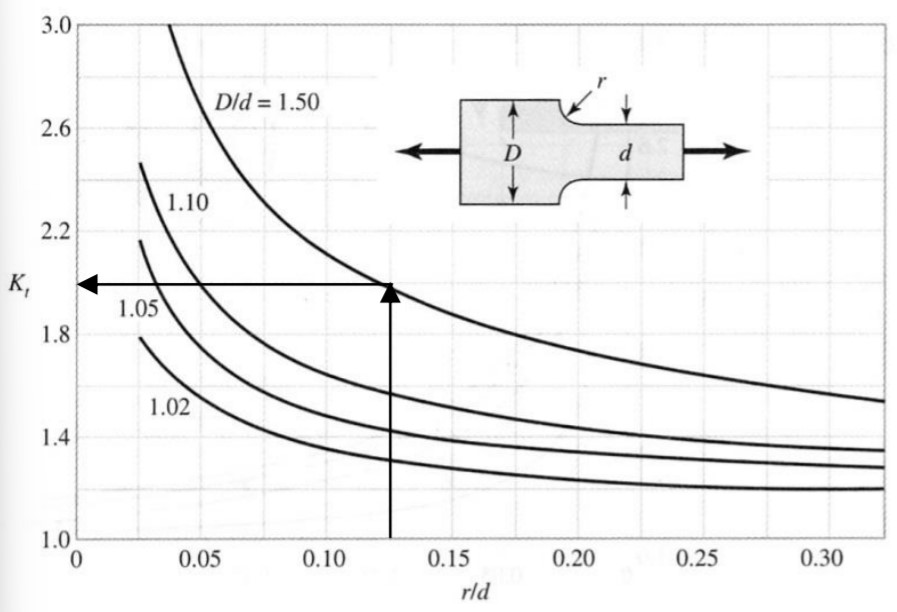
\includegraphics[width=7cm]{conc-factor-axial} \caption{}
		\end{subfigure}
		\begin{subfigure}{0.48\linewidth}
			\centering 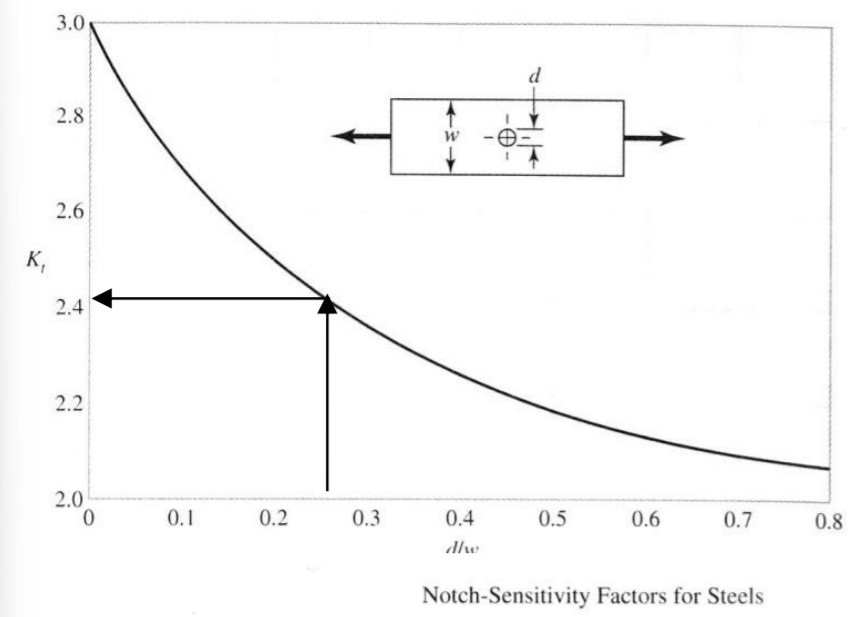
\includegraphics[width=7cm]{conc-factor-notch} \caption{}
		\end{subfigure}
		\caption{stress intensity factor $K_t$ for shouldered shaft (a) and notched plates (b) subjected to axial loadings.} \label{ex:fatiguekt}
	\end{figure}
	
	\begin{SCfigure}[1][bt]
		\centering 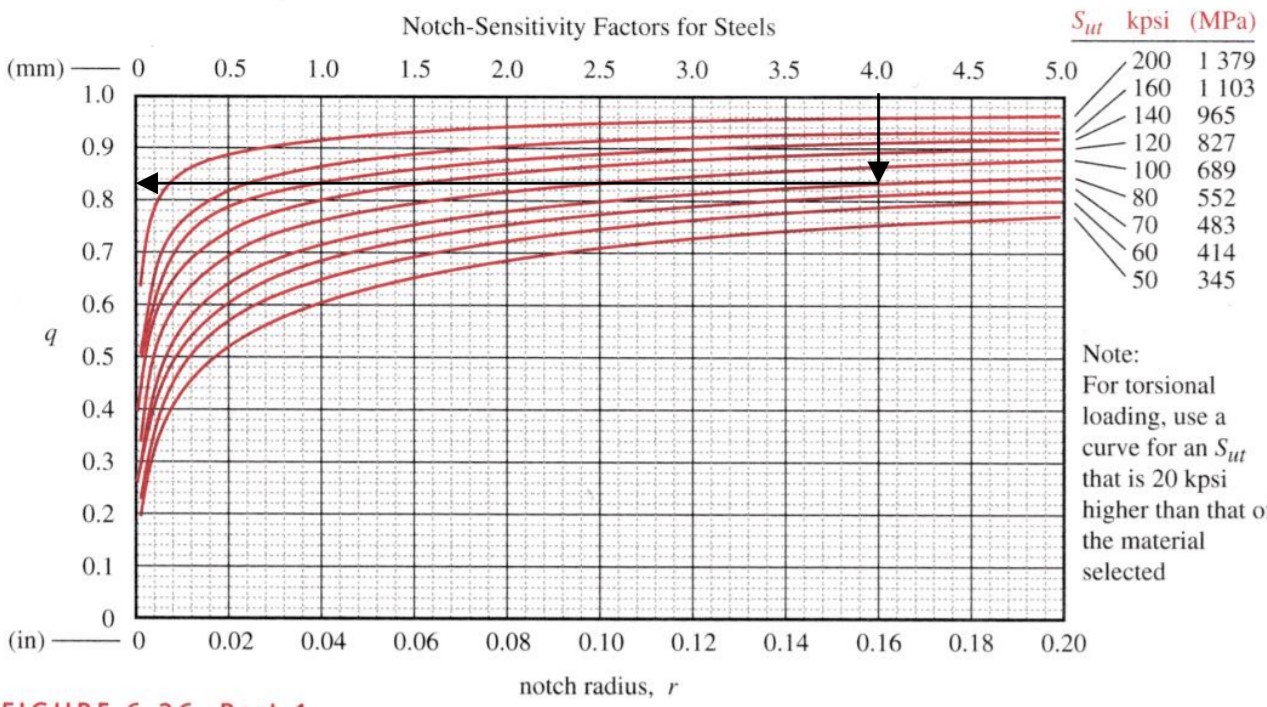
\includegraphics[width=9cm]{notch-sensitivity}
		\caption{notch sensitivity.} \label{ex:fatiguesensitivity}
	\end{SCfigure}
	
	To consider the mean stress effect we can use equation \ref{eq:plasticization} that's based on the assumption that if the notch root undergoes plasticization during the early strain cycle, thus stabilizing the cycle to a lower mean stress. Considering that $ K_t \sigma_{max,AA} = 150 MPa < \sys$ and $K_t \sigma_{max,BB} = 160 MPa \leq \sys$ than the following mean stress values should be used for the fatigue verification:
	\[ \sigma_{m,AA} = K_{f,AA} \sigma_{m,nom,AA} =75.06 MPa \qquad \sigma_{a,AA} = K_{f,AA} \sigma_{a,nom,AA} = 61.43 MPa \]
	\[ \sigma_{m,BB} = K_{f,BB} \sigma_{m,nom,BB} =79.27 MPa \qquad \sigma_{a,BB} = K_{f,BB} \sigma_{a,nom,BB} = 64.86 MPa \]
	
	Using Sodeberg's equation for the isocritical stress (more conservative approach) it's possible to determine the equivalent isocritically fully-reversed amplitude $\sigma_a^*$ as
	\[ \frac{K_f \sigma_a}{\sigma_a^*} + \frac{K_f \sigma_m}{\sys} = 1 \qquad \Rightarrow \quad \sigma_a^* = K_f \sigma_a \frac{\sys}{\sys - K_f \sigma_m} \]
	determining the values $\sigma_{a,AA}^* = 76.5MPa$ and $\sigma_{a,BB}^* = 80.8MPa$.
	
	To carry on the fatigue analysis it's necessary to compute the allowable stress $\sall$ depending on various coefficients. From equation \ref{eq:surfacefinish} the surface finish factor $C_s$ can be computed considering equation $a \suts ^b$ where the parameters $a = 4.51, b = -0.265$ are retrieved from table \ref{tab:surfacefinish} considering that the pieced is machined; this gives $C_s = 4.51 \cdot 550^{-0.265} = 0.85$. Considering that the action are axial, the loading coefficient is so $C_l = 0.7$. The dimension coefficient $C_d$ is instead different for the two section and depends on their equivalent diameter 
	\[ d_{eq,AA} = \sqrt{\frac 4 \pi bh } = 14.3 mm \hspace{3cm} d_{eq,BB} = \sqrt{\frac 4 \pi b (H-d)} = 15.1mm \]
	Considering equation \ref{eq:dimensioncoefficient} it can be noted that the dimension coefficient $C_d$ is approximately equal for both cases to $1.189\cdot 14.3^{0.097} \approx 1.189\cdot 15.1^{-0.097} \approx 0.92$. With that said the allowable stress is
	\[ \sall = \frac{C_s C_d C_l }{\phi} \sigma_{lim} = \frac{180.2}{\phi} MPa \]
	Equating $\sall = \sigma_a^*$ and solving for $\phi$ gives the safety factors for infinite fatigue life for both critical sections:
	\[ \phi_{AA} = \frac{180.2MPa}{\sigma_{a,AA}^*} = 2.53 \hspace{3cm} \phi_{BB} = \frac{180.2MPa}{\sigma_{a,BB}^*} = 2.39 \]
	
	\vspace{3mm}
	Considering now the case of variable amplitude effects, a linear damage accumulation model should be used; in this part only section BB will be discussed due to her being more critical than AA. Knowing the area $A = b(H-d) = 180mm^2$, as in the previous case, it has been possible to compute the maximum, minimum, mean and amplitude stress of the piece for each load condition:
	\[ F_m = \frac{F_{max} + F_{min}}{2} \qquad F_a = \frac{F_{max} - F_{min}}{2} \qquad \Rightarrow \qquad \sigma_m = \frac{F_m}{A} \quad \sigma_a = \frac{F_a}{A} \quad \sigma_{max} = \frac{F_{max}}{A} \]
	Each condition has been then converted into an isocritical alternating cycles following the rule
	\[ \frac{\sa}{\sa^*} + \frac{\sm}{\sys}  = 1 \qquad \Rightarrow \qquad \sa^* = \sa \frac{\sys}{\sys-\sm}\]
	With the data given from the starting table we have	
	\begin{center}
		\begin{tabular}{ c M{2cm} M{2cm} | M{2cm} M{2cm} M{2cm} }
			&  $F_m [N]$ &  $F_a[N]$ & $\sigma_m [MPa]$ & $\sigma_a [MPa]$ & $\sa^* [MPa]$ \\ \hline
			\#1 & 8500 & 9500 & 47.22 &  52.78 & 60.27\\
			\#2 & 12000 & 14000 & 66.67 & 77.78 & 94.32 \\
			\#3 & 14600 & 13400 & 81.11 & 74.44 & 94.65  \\
			\#4 & 15500 & 14500 & 86.11 & 80.56 & 104.16 \\
			\#5 & 16500 & 16000 & 91.67 & 88.89 & 117.15
		\end{tabular}
	\end{center} \noindent
	\begin{SCfigure}[1][b]
		\centering 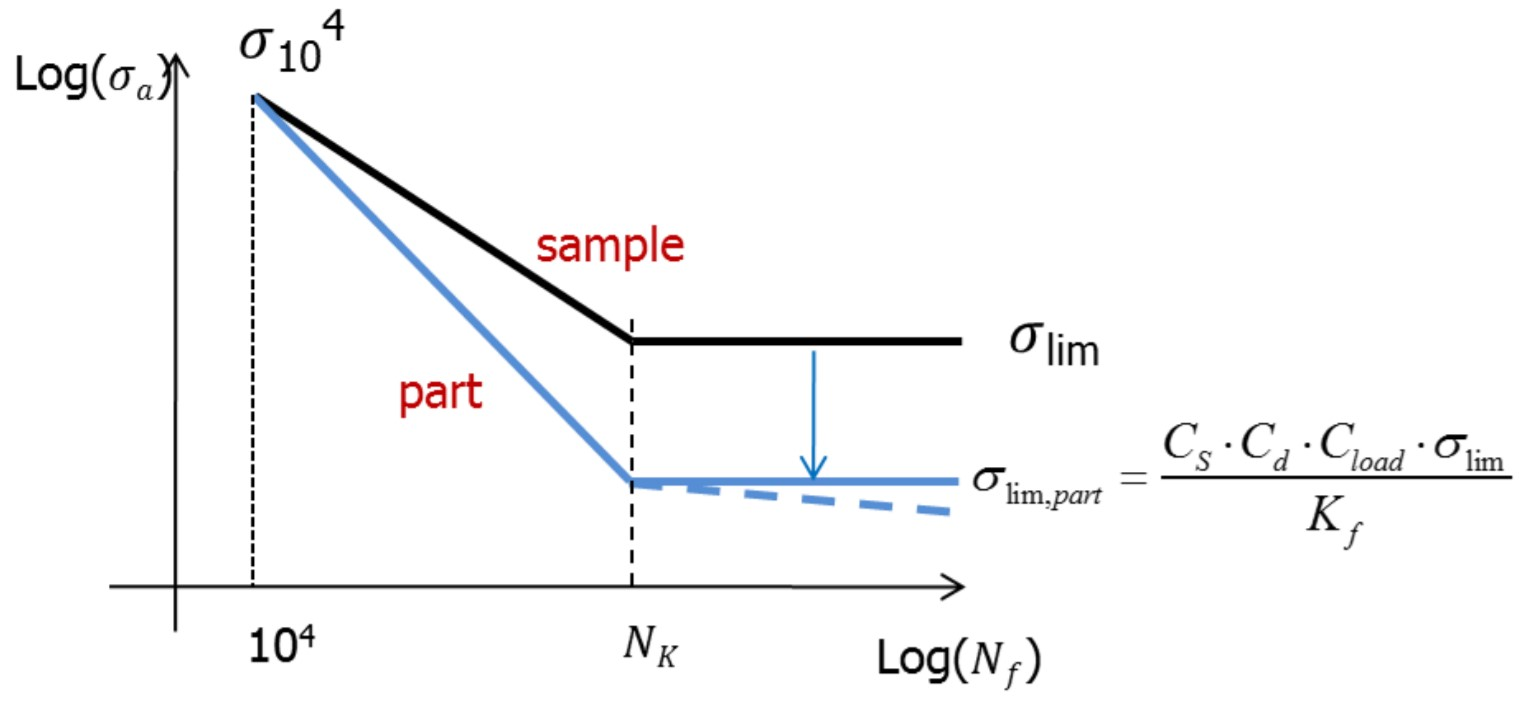
\includegraphics[width=9cm]{notch-effect}
		\caption{sample vs part SN curves.} \label{ex:notcheffetc}
	\end{SCfigure}
	
	As shown in figure \ref{ex:notcheffetc}, the notch effect has to be used to weaken the SN curve of the actual part respect to the theoretical values of the laboratory samples; in particular we have that
	\[ \sigma_{lim,part} = \frac{C_sC_dC_l}{K_f} \sigma_{lim} = 83.4 MPa \]
	Knowing the 50\% failure probability SN curve determined by the equation	
	\[ \sigma_a = \begin{cases}
		330MPa &  N_f > 2\cdot 10^6 \\
		1\,220 N_f^{-0.09} \qquad & 10^4 < N_f < 2\cdot 10^6
	\end{cases} \]
	and so having $\sigma_{10^4} = 1220 (10^4)^{-0.09} = 532.5MPa$ it's possible to compute the two parameter $1/k,C$ of the Basquin law (equation \ref{eq:basquin}) as
	\[\frac 1 k = \frac{-\log \left( \frac{\sigma_{lim}}{\sigma_{10^4}} \right)}{\log\left( \frac{N_{lim}}{10^4} \right)} = 0.35 \qquad \qquad \qquad C = \frac{\sigma_{10^4}}{\big(10^4\big)^{-1/k} } = 13\,369\]
	With that the SN curve of the actual part can be regarded as
	\[ \sigma_a = \begin{cases}
		83.4 MPa &  N_f > 2\cdot 10^6 \\
		13\,369 N_f^{-0.35} \qquad & 10^4 < N_f < 2\cdot 10^6
	\end{cases} \]
	Such system however doesn't take into account the damage of cycles in case of $\sa^* < 83.4MPa$ (infinite life due to having loads lower than the limit of the piece) while in reality they might increase the fatigue crack propagation generated by higher amplitude stress cycles. Such problem can be modelled considering a non-zero slope on the SN curve after $N_{lim}$, but with a coefficient $1/k'$ where
	\[ k = \frac 1{0.35} = 2.86 \qquad \Rightarrow k' = 2k-1=4.71 \qquad \Rightarrow \frac 1 {k'} = 0.212 \]	
	and a new constant $C'$ to match boundary condition described by
	\[ C' = \frac{83.4}{\big( 2\cdot 10^6\big)^{-1/k'}} = 1809 MPa \]
	And so the SN curve becomes
	\[ \sigma_a = \begin{cases}
		13\,369 N_f^{-0.35} \qquad & 10^4 < N_f < 2\cdot 10^6 \\
		1\,809 N_f^{-0.212} &  N_f > 2\cdot 10^6 
	\end{cases} \qquad \Rightarrow N_f = \left\{\begin{aligned}
		& \sqrt[-0.35]{\frac{\sa}{13\,369}} \qquad &&  \textrm{if } \sa >83.4MPa \\
		& \sqrt[-0.212]{\frac{\sa}{1\,809}} \qquad &&  \textrm{if } \sa < 83.4MPa \\		
	\end{aligned}\right.\]
	The damage $D_i$ for each hour of operation can so be regarded as $n_i/N_{f,i}$ and considering the values we have
	\begin{center}
		\begin{tabular}{ c M{2cm} M{2cm} M{2cm} | M{2cm} M{2cm} }
			&  $F_{min} [N]$ &  $F_{max}[N]$ & $n [\textrm{cycle}/h]$ & failure cycles $N_f$ & damage $D_i$ \\ \hline
			\#1 & -1000 & 18000 & 2000 & $9.30 \cdot 10^6$ & $2.15\cdot10^{-4}$ \\
			\#2 & -2000 & 26000& 1000 & $1.40 \cdot 10^6$ & $7.13\cdot10^{-4}$ \\
			\#3 & 1200 & 28000 & 500 & $1.39 \cdot 10^6$ & $3.60\cdot10^{-4}$ \\
			\#4 & 1000 & 30000 & 300 & $1.06 \cdot 10^6$ & $2.84\cdot10^{-4}$ \\
			\#5 & 500 & 32500 & 100 & $0.76 \cdot 10^6$ & $1.32\cdot10^{-4}$ \\ \hline
			\multicolumn{5}{r}{total damage $D_{tot}$:} & $17\cdot 10^{-4}$
		\end{tabular}
	\end{center}
	Finally we can estimate the number of operating hours of the part as
	\[ h = \frac 1 {D_{tot}} = 587 h \]
	
	
	
	
	
	
	
	
	
	
	
	
	
	
	
	
	
	
	
	
	
	
	
	